\documentclass[man]{apa7}
\usepackage[T1]{fontenc}
\usepackage[american]{babel}
\usepackage[style=apa,backend=biber]{biblatex}
\usepackage{csquotes}
\addbibresource{CountDominance.bib}

\title{Relative importance analysis for count regression models}
\author{Joseph N. Luchman}
\affiliation{Fors Marsh}
\leftheader{Luchman}
\shorttitle{Count Model Dominance}
\authornote{\addORCIDlink{Joseph N. Luchman}{0000-0002-8886-9717}. The author has read and approved the final version of the manuscript, has no conflicts of interest with respect to his authorship or the publication of this article, and did not receive or benefit from fundings of this article.}

\abstract{
	Count variables are common in behavioral science as an outcome. 
	Count regression models, such as Poisson regression, are recommended when analyzing count variables but can be challenging to interpret given their non-linear functional form. 
	I recommend relative importance analysis as a method to use in interpreting count regression model results. 
	This work extends on past research by describing an approach to determining the importance of independent variables in count regression models using dominance analysis (DA). 
	In this manuscript, I review DA as a relative importance method, recommend a pseudo-$R^2$ to use with count regression model-based DA, and outline the results of an analysis with simulated data that uses the recommended methodology. 
	This work contributes to the literature by extending DA to count regression models and provides a thoroughly documented example analysis that researchers can use to implement the methodology in their research.
}

\keywords{Dominance Analysis, Relative Importance, Poisson Regression, R-square, Negative Binomial Regression, Count Data}
	
\begin{document}

\maketitle

	Behavioral scientists often use how many times a behavior is observed as an outcome to answer research questions. 
	Such behavior counts arise from many different sources among aggreates or collectives of people and individuals over time.
	Aggregate behavior counts used in the literature include the number of organizations adopting a specific practice in a week \parencite{naumovska2021strength} and number of divestitures organizations make in a year \parencite{bettinazzi2021stakeholder}. 
	Individual-level behavior counts used in the literature include the number of scientific articles published in a year among scholars \parencite{rotolo2013does} or number of errors that resulted in an accident in the last three months among medical doctors \parencite{naveh2015active}.
	Behavior counts such as the above examples are valuable outcomes given that behavioral science concepts are often defined terms of behavior \parencite[e.g., job performance;][]{motowidlo2003job} and strategies to validate outcomes often use observable behavior as an outcome \parencite[e.g., criterion-oriented validity;][]{cronbach1955construct}.
	
	However valuable as outcomes, behavior counts as a dependent variable in data analysis require the use of specialized tools.
	The recommended data analysis strategy with behavior counts uses regression models designed for non-negative integer or count distributions \parencite[e.g.,][]{blevins2015count}.
	These count regression models include the Poisson regression and negative Binomial regression models.
	Both Poisson regression and negative Binomial regression are commonly used in the behavioral science literature and implemented in many data analytic software environments.
	
	Count regression models are generalized linear models that transform the predictive equation to ensure that predicted values stay in the range of the depemdent variable.
	Count regression models use an exponential or log-linear transformation that has the form $y = e^{\beta}$. 
	Thus, the predictive equation represented by $\beta$ requires back-transformation using a natural logarithm in order to obtain a predicted count value.
	This log-linear transformation ensures that the linear predictrd values can take on any real number yet, when back-transformed into predicted counts, will have a lower bound of 0.
	
	Count regression model results are challenging to interpret directly.
	This is because count regression model coefficients describe how the natural logarithm of the dependent variable changes given a 1 unit change to an independent variable. 
	When back-translated through an exponential function, count regression model coefficients are known as incidence rate ratios and describe the percentage change in the dependent variable per unit change to the independent variable.
	Because IRRs describe percentage change, count regression model coefficients produce predicted values that are relative or change in their magnitude over the continuum of the dependent variable.
	For example, a count regression model coefficient does not differentiate between a change from 1 predicted behavior to 2 and 5 predicted behaviors to 10. 
	Despite the noteworthy difference in the absolute number of behaviors in both examples, each describe a 100\% increase.
		
	Model post-estimation methods such as graphing estimated marginal means are useful interpretive tools for log-linear count regression models as they help to contextualize the count regression models' predicted values.
	Another increasingly common model post-estimation tool used to contextualize model predictions is relative importance analysis \parencite{tonidandel2011relative}. 
	Relative importance analysis is used to compare how each independent variable in the model contributes to a model fit metric such as the $R^2$ and is commonly implemented using dominance analysis/DA \parencite{azen2003dominance}.
	
	Published methodological work has extended DA from the linear regression model/LRM on which it was originally developed, to other linear models including binary \parencite{azen2009using}, ordered, and multinomial logit models \parencite{luchman2014relative}.	
	This work extends DA to count regression models and, in so doing, makes two contributions to the literature.
	This work first reviews DA as a relative importance methodology, recommends using a specific pseudo-$R^2$ statistic for count regression model-based DA, and implements a data analytic example of DA.

	Second, this paper extends on the work of Blevins, Tsang, and Spain \parencite*{blevins2015count} who review and offer multiple recommendations for the application of count regression models to research questions in behavioral science. 
	Blevins et al. describe model and analytic details about the Poisson regression and negative Binomial regression models and provide a flowchart that researchers can use to identify which count regression model might be best to choose for their data analysis.
	In this work, I extend on their review to add an in-depth discussion of DA and its role as a post-estimation methodology.
	DA extends on the interpretation of coefficients to describe how the coefficients, when applied to the observed data, improve model-to-data fit in predicting the count dependent variable.

	I begin the manuscript with a discussion of the conceptual background of DA.
	The conceptual discussion of DA focuses on outlining three different levels of dominance between independent variables, how these levels of dominance are determined in the data, and what each level of dominance means in terms of independent variable importance.
	The next section recommends a fit metric to apply to count regression models for the purpose of determinining importance using DA.
	In this count regression model focused section, I draw parallels between the explained variance $R^2$ used by the LRM as a fit metric and an analogous fit metric for count regression models that is particularly useful for DA.
	Finally, I describe an extensive data analytic example.
	This final section uses simulated data to estimate a Poisson regression model and a Poisson regression model-based DA where the methods described in the previous two sections are applied.
		
\section{Dominance Analysis}

	Behavioral scientists have used many methods over the years to determine how important an independent variable is in a LRM \parencite[see reviews in][]{gromping2007estimators, johnson2004history}.
	Methods for determining the importance of an independent variable have ranged from the use of a correlation coefficient between the independent variable and dependent variable, to the independent variable's standardized regression coefficient, to the increment the independent variable makes to the $R^2$ over and above other independent variables.
	These methods, however informative in specific circumstances, make assumptions about an independent variable's contribution to prediction.
	These methods assume in some cases that an independent variable's contribution should not be adjusted for other independent variables (i.e., the correlation coefficient) and in other cases that the adjustment should occur only after all other independent variables are included (i.e., incremental $R^2$, standardized coefficient).
	In most situations, independent variable inclusion ordering is arbitrary and as opposed to choosing one approach or the other, recommended importance methods should account for different bi- and multivariate relationships with the dependent variable \parencite{johnson2004history}.
	The most conceptually useful importance methods then produce determinations that are independent of independent variable inclusion order.
	
	DA is a method for determining independent variable importance independent of inclusion order that was originally developed for the LRM by Budescu \parencite*{budescu1993dominance}.
	DA extended on previously proposed methods by defining importance in terms of pairwise independent variable comparisons across $R^2$ values associated with multiple sub-models.
	An LRM with $p$ independent variables produces total of $2^p$ sub-models corresponding to all possible combinations of independent variables included or excluded from estimation.
	DA achieves order independence in the importance determiniations it makes by comparing the $R^2$ values associated with the two focal, comparison independent variables' across all sub-models that include combinations of non-focal, other independent variables. 
	A non-focal independent variable sub-model is one that contains a distinct subset of the $p - 2$ independent variables that are not the focus of the comparison.
	The $\emptyset$ or a sub-model that includes no non-focal independent variables, is also a possible sub-model used in these comparisons.	
	In this way, the dominance comparisons do not depend on the order of independent variable inclusion and require that one of the focal, comparison independent variables obtain a higher $R^2$ value than the other focal independent variable across all sub-models---that is, irrespective of the order in which the independent variable is included in the model.
	
	As an example of how the dominance comparison is implemented, consider a model with 4 independent variables: $IV_x$, $IV_z$, $IV_w$ and $IV_v$ predicting $Y$.
	If I am comparing $IV_x$ and $IV_z$, there would be a total of four possible $R^2$ comparisons, each of which is reported below in Table \ref{tab:exdom}.
	In each comparison, the subscripted model indicates the LRM prediction equation in symbolic form.
	The terms in braces include the other, non-focal independent variable subset across which both of the focal, comparison independent variables are being evaluated.
	$IV_x$ dominates $IV_z$ only when all the $R^2$ values for sub-models that include $IV_x$ are greater than the $R^2$ values for sub-models that include $IV_z$.
	The dominance comparisons described in this section are known as complete dominance and are recognized as the most stringent, or hardest to achieve, dominance designation that an independent variable can have over another independent variable \parencite{azen2003dominance}.	

		\begin{table}[h!]
			\centering
			\caption{\centering Example Dominance Comparisons}
			\begin{tabular}{ l | l l }
				
				& Sub-model with $IV_x$ & Sub-model with $IV_z$ \\
				\hline
				Across null set/no other independent variables & $R^2_{Y \sim IV_x + \{\emptyset\}}$ & $R^2_{Y \sim IV_z+ \{\emptyset\} }$ \\
				Comparing across $IV_w$ & $R^2_{Y \sim IV_x + \{IV_w\}}$ & $R^2_{Y \sim IV_z + \{IV_w\}}$ \\
				Comparing across $IV_v$ & $R^2_{Y \sim IV_x + \{IV_v\}}$ & $R^2_{Y \sim IV_z + \{IV_w\}}$ \\
				Comparing across both $IV_w$ and $IV_v$ & $R^2_{Y \sim IV_x + \{IV_w + IV_v\}}$ & $R^2_{Y \sim IV_z + \{IV_w + IV_v\}}$ \\
				\hline
		\end{tabular}
		\label{tab:exdom}
	\end{table}
	
	\subsection{Complete Dominance}
	
	Complete dominance is the most stringent of the dominance designations as it is a difficult designation for an independent variable to achieve over another.
	Complete dominance is difficult to achieve as it involves direct comparisons between independent variable pairs across multiple sub-model $R^2$ values and is non-compensatory; all sub-model $R^2$ value comparisons must show that one independent variable has a larger value than the other independent variable or the designation will fail to be achieved.
	
	The process for determining complete dominance between a pair of independent variables, for example $IV_x$ and $IV_z$, with an arbitrary number of non-focal independent variables in the model ($p - 2$) proceeds as:
	\begin{equation}
		IV_x \, D \, IV_z \quad if \quad 2^{p-2} = \sum^{2^{p-2}}_{j=1} \Biggr\{ 
		\begin{array}{l}
			if \ R^2_{Y \sim IV_x + \{u_j\}} > R^2_{Y \sim IV_z + \{u_j\}} \ then \ 1 \\
			else \ 0 
		\end{array}
		\label{eq:cptdom}
	\end{equation}
	Where $u_j$ is a distinct subset of the other $p - 2$ independent variables.
	As in Table \ref{tab:exdom}, the braces surrounding $u_j$ indicate that it is a subset of non-focal independent variables.
	The $D$ in this case is a designation indicating complete dominance of $IV_x$ over $IV_z$.
	Ultimately, if $IV_x$ completely dominates $IV_z$ as is outlined in Equation \ref{eq:cptdom}, $IV_x$ is clearly and unconditionally better than $IV_z$ in terms of explaining variance in $Y$ given the LRM from which all sub-models were derived.	
	
	Because complete dominance is a difficult criterion to achieve in comparing independent variable pairs, alternative and more compensatory, dominance designations have been proposed to provide more ways to compare the predictive usefulness of independent variables against one another.
	As I will discuss, the alternative dominance designations involve averaging the $R^2$ increment values associated with each independent variable and determining importance by comparing those average values.
	
	\subsection{Conditional Dominance}
	
	A less stringent dominance designation between independent variable pairs than complete dominance is called conditional dominance.
	Conditional dominance relaxes the stringency of the comparisons across pairs of independent variables by evaluating how each independent variable contributes to the $R^2$, on average, when they are included in every relative position in the model.
	
	By comparing averages of $R^2$ increments by relative position, conditional dominance allows some sub-models with higher $R^2$ increment values at a specific inclusion order for $IV_x$ compared to $IV_z$ to compensate for sub-models with lower $R^2$ increment values for $IV_x$ compared to $IV_z$ at that same order.
	This compensatory property of the averages by inclusion order makes conditional dominance a less stringent criterion and makes it more likely to obtain a dominance designation.
	
	The average increments to the $R^2$ used to determine conditional dominance are known as conditional dominance statistics.
	Because each independent variable can be included at any relative position in the model, in a model with $p$ independent variables, each independent variable will have $p$ conditional dominance statistics to compare to another independent variable.
	Extending on Table \ref{tab:exdom}, determining conditional dominance between $IV_x$ and $IV_z$ would involve all four different conditional dominance statistics, the computation of which are outlined below in Table \ref{tab:excdl}.
	
	\begin{table}[h!]
		\centering
		\caption{\centering Example Conditional Dominance}
		\begin{tabular}{ l | l l }
			Comparing at & Average with $IV_x$ & Average with $IV_z$ \\
			\hline
			One independent variable & $\Delta R^2_{Y \sim IV_x + \{\emptyset\}}$ & $\Delta R^2_{Y \sim IV_z + \{\emptyset\}}$ \\
			\hline
			& $(\Delta R^2_{Y \sim IV_x + \{IV_w\}} + $ & $(\Delta R^2_{Y \sim IV_z + \{IV_w\}} + $ \\
			Two independent variables & $\Delta R^2_{Y \sim IV_x + \{IV_v\}} + $ & $\Delta R^2_{Y \sim IV_z + \{IV_v\}} + $ \\
			& $\Delta R^2_{Y \sim IV_x + \{IV_z\}})\frac{1}{3}$ & $\Delta R^2_{Y \sim IV_z + \{IV_x\}})\frac{1}{3} $ \\
			\hline
			& $(\Delta R^2_{Y \sim IV_x + \{IV_w + IV_v\}} + $ & $(\Delta R^2_{Y \sim IV_z + \{IV_w + IV_v\}} + $ \\
			Three independent variables & $\Delta R^2_{Y \sim IV_x + \{IV_w + IV_z\}} + $ & $\Delta R^2_{Y \sim IV_z + \{IV_w + IV_x\}} + $ \\
			& $\Delta R^2_{Y \sim IV_x - \{IV_v + IV_z\}})\frac{1}{3}$ & $\Delta R^2_{Y \sim IV_z + \{IV_v + IV_x\}})\frac{1}{3}$ \\
			\hline
			Four independent variables & $\Delta R^2_{Y \sim IV_x + \{IV_w + IV_v + IV_z\}}$ & $\Delta R^2_{Y \sim IV_z + \{IV_w + IV_v + IV_x\}}$ \\
			\hline
		\end{tabular}
		\label{tab:excdl}
	\end{table}
	
	The $\Delta$ used in Table \ref{tab:excdl} indicates that the $R^2$ value is an increment made by the focal independent variable beyond the subset of non-focal independent variables in braces.
	Note that the conditional dominance statistics use $R^2$ increments from subsets that include all other non-focal independent variables.
	Hence, conditional dominance comparisons between two independent variables will include increments from the independent variable against which they are being compared in their average value.
	This is a noteworthy difference from complete dominance designations that do not use sub-model $R^2$ values that include the independent variable against which the focal independent variable is being compared.
	
	The process of computing conditional dominance statistics for $IV_x$ with $i$ independent variables in the sub-model is defined as in Equation \ref{eq:cdlst} below.
	\begin{equation}
		C^{i}_{IV_x} = \frac{\sum^{k_i}_{g=1} \Delta R^2_{IV_x + \{o_g\}}}{k_g}
		\label{eq:cdlst}
	\end{equation}
	Where $k_i$ is the number of combinations of size $i$ given $p$ independent variables and $o_g$ is a distinct subset of the $p - 1$ independent variables of size $i - 1$ that are included in the sub-model.	
	Determining conditional dominance between $IV_x$ and $IV_z$ proceeds as in Equation \ref{eq:cdldom}.
	\begin{equation}
		IV_x \ D_c \ IV_z \quad if \quad p = \sum^p_{i=1} \Biggl\{ 
		\begin{array}{l}
			if \ C^{i}_{IV_x} > C^{i}_{IV_z} \ then \ 1 \\ 
			else \ 0 
		\end{array}
		\label{eq:cdldom}
	\end{equation}
	Where $D_c$ is a designation indicating conditional dominance of $IV_x$ over $IV_z$.	
	When $IV_x$ does not completely but does conditionally dominate $IV_z$, $IV_x$ is generally better than $IV_z$ for explaining variance in $Y$ given the underlying LRM irrespective of inclusion order in the model.
	Conditional dominance thus suggests that $IV_x$'s explanatory value is generally higher than $IV_z$ when considering their values at the same inclusion orders.
	
	Conditional dominance between an independent variable pair is less stringent than complete dominance but can still be a difficult designation to meet in models with a great deal of between-independent variable overlap.
	As a result, a third dominance designation was developed that involves yet another averaging step as is described in the next section.
	
	\subsection{General Dominance}
	
	The least stringent dominance designation between independent variable pairs is called general dominance.
	General dominance further relaxes the stringency of the comparisons between independent variable pairs by changing the focus from comparing average increments grouped by the number of independent variables in a sub-model to the arithmetic average of these averages.
	General dominance is then the average of the conditional dominance statistics for each independent variable.
	By averaging over conditional dominance statistics, general dominance allows higher contributions at specific numbers of independent variables in the sub-model to compensate for lower contributions at other numbers of independent variables in the sub-model. 
	The values generated by general dominance will, in almost all cases, produce a dominance designation between the pair of independent variables.
	
	The averaged conditional dominance statistics computed for determining general dominance are known as general dominance statistics. 
	Table \ref{tab:exgen} shows the general dominance statistic computation for $IV_x$ and $IV_z$.
	This computation incorporates all the values in Table \ref{tab:excdl} but summed into a single statistic.
	
		\begin{table}[h!]
		\centering
		\caption{\centering Example General Dominance}
		\begin{tabular}{ l l }
			Average with $IV_x$ & Average with $IV_z$ \\
			\hline
			$\Delta R^2_{Y \sim IV_x + \{\emptyset\}}\frac{1}{4} + $ & $\Delta R^2_{Y \sim IV_z + \{\emptyset\}}\frac{1}{4} +$ \\
			$(\Delta R^2_{Y \sim IV_x + \{IV_w\}} + $ & $(\Delta R^2_{Y \sim IV_z + \{IV_w\}} + $ \\
			$\Delta R^2_{Y \sim IV_x + \{IV_v\}} + $ & $\Delta R^2_{Y \sim IV_z + \{IV_v\}} + $ \\
			$\Delta R^2_{Y \sim IV_x + \{IV_z\}})\frac{1}{12} + $ & $\Delta R^2_{Y \sim IV_z + \{IV_x\}})\frac{1}{12} + $ \\
			$(\Delta R^2_{Y \sim IV_x + \{IV_w + IV_v\}} + $ & $(\Delta R^2_{Y \sim IV_z + \{IV_w + IV_v\}} + $ \\
			$\Delta R^2_{Y \sim IV_x + \{IV_w + IV_z\}} + $ & $\Delta R^2_{Y \sim IV_z + \{IV_w + IV_x\}} + $ \\
			$\Delta R^2_{Y \sim IV_x - \{IV_v + IV_z\}})\frac{1}{12} + $ & $\Delta R^2_{Y \sim IV_z + \{IV_v + IV_x\}})\frac{1}{12} +$ \\
			$\Delta R^2_{Y \sim IV_x + \{IV_w + IV_v + IV_z\}}\frac{1}{4}$ & $\Delta R^2_{Y \sim IV_z + \{IV_w + IV_v + IV_x\}}\frac{1}{4}$ \\
			\hline
		\end{tabular}
		\label{tab:exgen}
	\end{table}

	As is implied by the computations in Table \ref{tab:exgen}, general dominance statistics are a weighted average of the individual increments to the $R^2$s and is defined for $IV_x$ in Equation \ref{eq:genst}.
	\begin{equation}
		C_{IV_x} = \frac{\sum^{p}_{i=1} C^i_{IV_x}}{p}
		\label{eq:genst}
	\end{equation}
	Using the general dominance statistics computed in Equation \ref{eq:genst}, determining whether $IV_x$ generally dominates $IV_z$ is proceeds as in Equation \ref{eq:gendom}.
	\begin{equation}
		IV_x \ D_g \ IV_z \quad if \quad C_{IV_x} > C_{IV_z}
		\label{eq:gendom}
	\end{equation}
	Where $D_g$ is a designation indicating general dominance of $IV_x$ over $IV_z$.	
	When $IV_x$ does not completely or conditionally but does generally dominate $IV_z$, $IV_x$ is generally better than $IV_z$ for explaining variance in $Y$ given the underlying LRM but is sensitive to inclusion order in the model.
	General dominance thus suggests that $IV_x$'s predictive usefulness is, on average, better than $IV_z$ and that it is more important when not directly considering the effects of independent variable inclusion order.
	
	Note that the general dominance statistic values, when summed across the $p$ independent variables, equals the sub-model $R^2$ when all $p$ independent variables are included.
	This is a useful feature of the general dominance statistics that, as has been discussed in other reviews \parencite{gromping2007estimators,johnson2004history}, ties this method to earlier work on independent variable importance which focused on the decomposition of the $R^2$ statistic.

	In the sections above, I have provided a brief discussion of the conceptual development of the DA method, reviewed how DA statistics are computed, and reviewed how importance for independent variables is determined.
	In the section below, I transition from a broad outline of DA to a more targeted discussion on application of DA to count regression models.
	The focus of the next section is on a discussion of count regression model-based DA with attention to considering which fit statistic should be used when applying DA to count regression models.
	
\section{Applying Dominance Analysis to Count Regression Models}

	A complication of applying DA to count regression models is that the literature on DA has generally focused on how to apply the method to the LRM with the variance explained $R^2$ as a fit statistic.
	Given the semi-continuous nature of count dependent variables and that the predicted values from count regression models are typically in the form of a non-negative rational number, it is possible to use the explained variance $R^2$ when determining importance with a count regression model.
	
	Although the variance explained $R^2$ could be applied to count regression models, there are good conceptual reasons to choose another fit statistic. 
	In the section below, I provide a rationale for the choice of a different metric, the deviance $R^2$ or $R^2_{DEV}$, that better reflects the criteria underlying how count regression models fit to data. 
	
	\subsection{Count Regression Fit Statistic: Deviance $R^2$} 
	
	Statistical models are fit using information about the data as applied to a probability distribution to find their most likely parameter values.
	A fit statistic applied to evaluating the fit of a statistical model to data is also most useful when the computation of the statistic is conceptually aligned with the model that it is being used to evaluate.
	Thus, choosing a fit statistic that matches the underlying fitting criterion of statistical model's probability distribution will best reflect how the model fits to data.
	
	Consider that the explained variance $R^2$ is computed as $\frac{\sum (\bar{Y} - \hat{Y})^2}{\sum (Y - \bar{Y})^2} = \frac{SS_{model}}{SS_{total}}$ or the ratio of the variance of the predicted values (i.e., the model sums of squares; $SS_{model}$) over the variance of the predicted values (i.e., the total sums of squares; $SS_{total}$).
	The LRM is based on a Normal probability distribution and uses least-squares as its fitting criterion.
	Least squares seeks to minimize $SS_{residual} = \sum (Y - \hat{Y})^2$ or the residual sums of squares between the predicted values from the LRM and the observed dependent variable. 
	The $SS_{residual} = SS_{total} - SS_{model}$ and thus the explaned variance $R^2$ can also be computed as $1 - \frac{SS_{residual}}{SS_{total}}$.
	The explained variance $R^2$ is then closely tied to the LRM and its fitting criterion.
	It is important to note that the computation used to obtain the $SS_{residual}$ is also known as the deviance ($DEV$) for the Normal distribution as it describes how the model's predictions deviate from observed values \parencite{mccullagh2019generalized}.
	The $SS_{residual}$ is thus a $DEV_{model}$ or a model deviance for the LRM.
	
	The Poisson regression follows the Poisson distribution and the negative Binomial regression follows the negative Binomial distribution--both of which are probability distributions meant for discrete data like non-negative counts.
	For example, the deviance for Poisson regression and a special case of the negative Binomial regression\footnote{
		This special case is the negative Binomial regression estimated using a quasi-likelihood method. 
		Maximum likelihood methods require a more complex form given the estimation of the $\alpha$/$\delta$ parameter.} 
	is $\sum Y\ln \frac{Y}{\hat{Y}} - (Y - \hat{Y})$. 
	Note that this Poisson regression-focused deviance value differs from the Normal distribution deviance in that it tends to penalize underprediction more than overprediction.
	The extra penalties assigned to underprediction are consistent with the truncated, semi-continuous nature of count dependent variables in that they cannot go below 0 and, thus, tend to be penalized more heavily toward the conceptual lower bound of the distribution.
	By contrast, Normal distribution-based deviance has no such constraint and penalizes discrepancies from observed values equally in either direction.
	
	In considering a reasonable fit statistic to apply to count regression models given the differences between the underlying fitting criteria for the LRM and count regression models, Cameron and Windmeijer \parencite*{cameron1996r} devised the $R^2_{DEV}$ or deviance $R^2$ outlined in Equation \ref{eq:r2dev} below.
	\begin{equation}
		R^{2}_{DEV} = 1 - \frac{DEV_{model}}{DEV_{null}}
		\label{eq:r2dev}
	\end{equation}
	Where $DEV_{null}$ is the model deviance for an intercept- or mean-only model and is equivalent to $SS_{total}$ for an LRM.
	The $R^2_{DEV}$ is then a direct extension of the explained variance $R^2$ but is more flexibile in that it can be applied to count regression models when using their deviance computations.
	I recommend the use of $R^2_{DEV}$ with $DEV_{model}$ and $DEV_{null}$ values that are based on each count regression model's fitting criteria as a fit statistic for DA.
	
	The $R^2_{DEV}$ is a conceptually more reasonable choice than the explained variance $R^2$ for count regression model-based DA as, if a researcher applies the explained variance $R^2$ to a count regression model, they are applying a fit statistic that uses a deviance computation intended for the LRM to count regression models with very different fitting criteria. 
	Having outlined a rationale for the choice of a specific fit statistic to use when applying DA to count regression models, in the sections to follow I transition to an example application of the proposed methodology.
	The sections below briefly outline the data generated for this illustration, describe the models estimated from the data, and also describe how DA designations were determined.
	
	\subsection{Count Regression Model-based Dominance Analysis: An Analytic Example}
	
	The goal of this section was to provide an example analysis using the recommended $R^2_{DEV}$ count regression model-based DA methodology.
	This example was intended to be useful as a guide for researchers and analysts interested in applying this method to count regression models.
	In the section below, I began by describing how I generated data for the example based on a Poisson regression model\footnote{
		An example using a negative Binomial regression is available in the online supplement.}.
	The methods used to generate these data were not directly relevant to the goals of this manuscript and, as such, have been included in an online supplement.
	Please note that the online supplement outlines the code to generate the data and development perspective behind the generation of these data in great detail.
	The section below was focused primarily on describing the conceptual nature of the data so that the reader can follow along prior to transitioning to reporting on the primary analysis.

		\subsubsection{Data Generation}
	
	The fabricated data simulated and discussed in this work is related to a fabricated study on the number of solutions a student provides to personal relationship problem given 20 minutes to respond that met minimum criteria for quality of reasoning.
	The data generated for this study were collected from 6,780 simulated students.
	The study researchers expected that the number of personal relationship problem solutions reported by each simulated student would be Poisson distributed.
	
	The four independent variables used in the fabricated data were four survey scales that were normed such that the mean of each was roughly 0 and standard deviation was roughly 1. 
	The first scale used to predict the number of solutions reported was a cognitive ability, or intelligence, scale reflecting the respondent's congnitive capacity and skills.
	This scale is denoted $ability$ in the results.
	The second survey scale was solution motivation or the respondent's motivation to try to resolve the personal relationship problem.
	This scale is denoted $motivation$ in the results.
	The third survey scale was tactfulness or the extent to which the respondent is sensitive to social considerations.	
	This scale is denoted $tact$ in the results.
	The fourth survey scale was rhetorical skill or the skill with which the respondent can construct a convincing argument
	This scale is denoted $skill$ in the results.
	
	The means, standard deviations, and correlations between all four independent variables and two dependent variables are reported below in Table \ref{tab:desc}. 
	
	\begin{table}[h!]
		\centering
		\caption{\centering Descriptive Statistics} 
		\begin{tabular}{lrr|rrrrr}
			\hline 
			&  & Standard & \multicolumn{5}{c}{Correlations} \\ 
			Variable & Mean & Deviation & $ability$ & $motivation$ & $tact$ & $skill$ & $solutions$ \\ 
			\hline
			$ability$ & $-0.0355$ & $1.1853$ & $1.0000$ & $0.4168$ & $0.1446$ & $0.2180$ & $0.4175$ \\ 
			$motivation$ & $-0.0261$ & $1.4494$ & $0.4168$ & $1.0000$ & $0.1958$ & $0.2850$ & $0.3592$ \\ 
			$tact$ & $-0.0056$ & $1.5480$ & $0.1446$ & $0.1958$ & $1.0000$ & $0.3295$ & $0.2913$ \\ 
			$skill$ & $0.0144$ & $1.9211$ & $0.2180$ & $0.2850$ & $0.3295$ & $1.0000$ & $0.3726$ \\ 
			$solutions$ & $0.9940$ & $1.0082$ & $0.4175$ & $0.3592$ & $0.2913$ & $0.3726$ & $1.0000$ \\ 
			\hline 
		\end{tabular}
		\label{tab:desc}
	\end{table}
	
	Note that, on average, each of the simulated respondents produced a solution in the 20 minute period under study.
	Table \ref{tab:desc} also shows that the variance of the number of solutions produced was consistent with its expected underlying Poisson distribution.
	Specifically, solution production had a variance of 1 which closely matches the mean as is assumed of the Poisson distribution. 

		\subsubsection{Regression Results}
		
	The solution production dependent variable was Poisson distributed by design and could be modeled using a Poisson regression.
	The Poisson regression results using the four survey scale independent variables to predict solution counts were reported in Table \ref{tab:poisreg}. 
	Table \ref{tab:poisreg} included coefficients ($\beta$), standard errors ($\sigma_{\beta}$), 95\% confidence intervals, and exponentiated coefficients or incidence rate ratios/IRRs ($e^{\beta}$).
	
	\begin{table}[h!]
		\centering
		\caption{\centering Poisson Regression Predicting Relationship Problem Solutions Produced} 
		\begin{tabular}{l|rrrrr}
			\hline 
			\multicolumn{1}{l}{} &  &  & \multicolumn{2}{c}{95\% Confidence Interval} &   \\ 
			\multicolumn{1}{l}{} & $\beta$ & $\sigma_{\beta}$ & Low & High & $e^{\beta}$ \\ 
			\hline 
			$ability$ & $0.2431$ & $0.0114$ & $0.2208$ & $0.2655$ & $1.2753$ \\  
			$motivation$ & $0.1081$ & $0.0095$ & $0.0896$ & $0.1267$ & $1.1142$ \\ 
			$tact$ & $0.0999$ & $0.0083$ & $0.0835$ & $0.1162$ & $1.1050$ \\
			$skill$ & $0.1158$ & $0.0069$ & $0.1024$ & $0.1293$ & $1.1228$ \\ 
			$Intercept$ & $-0.1507$ & $0.0138$ & $-0.1780$ & $-0.1237$ & $0.8601$ \\
			\hline 
		\end{tabular}
		\label{tab:poisreg}
	\end{table}
	
	Table \ref{tab:poisreg} showed that each of the independent variables had a positive effect on the number of solutions produced and each appeared to be statistically significant (at the $p < .05$ level) as was implied by the confidence intervals not including the value of 0.
	
	In terms of coefficient magnitude, ability had the largest effect on the rate of solution production. 
	Each  standard deviation increase in the ability scale led to a 27.5\% increase in the solutions produced given the IRR value.
	Rhetorical skill obtained the second-largest effect on solution production rates.
	Each standard deviation increase on the skill scale led to a 12.3\% increase in the number of solutions produced given its IRR.
	Motivation and tact obtained the smallest increases in solution production.
	Motivation resulted in a 11.4\% increase and tact a 10.5\% increase in the number of solutions produced given their IRRs. 
	
	The IRR value for the model intercept represented the expected number of solutions produced when all independent variables were at their means of 0.
	Because each independent variable had a mean of 0, the model intercept represented the mean number of solutions produced. 
	Note that the .8601 value obtained was similar to the overall mean of solutions in Table \ref{tab:desc}.
	This .8601 value could also used as the baseline rate of solutions produced.
	For instance, the expected number of solutions produced for respondents who had an ability score that was one standard deviation above the mean, but had mean value on all other independent variables, was $.8601*1.2753 = 1.0969$ or just above 1 solution produced.
	As opposed to reporting on single values as I have above, plotting of marginal means across levels of different independent variables adds value to the model interpretation \parencite[see][for a similar perspective]{ronkko2022eight} and more clearly depicts the multiplicative effects produced by count regression models.
	Although I did not include marginal means plots in this manuscript for brevity, such plots were reported in the online supplement for interested readers.
	
	The Poisson regression modeling result reported in Table \ref{tab:poisreg} showed that all four independent variables had non-trivial predictive effects on solution production and, in addition, obtained different coefficient magnitudes.
	These different coefficient magnitudes, in combination with the different variances observed in Table \ref{tab:desc}, indicated likely differences in the importance of each independent variable for explaining solution production.
	
	In the section below, I transition to the focal analysis of this work where I determined the importance of each independent variable for predicing solution production using DA.
	In this way, the section below providds an empirical example that applied the designation and computational formulas in Equations \ref{eq:cptdom}, \ref{eq:cdlst}, \ref{eq:cdldom}, \ref{eq:genst}, and \ref{eq:gendom} to the Poisson regression model in Table \ref{tab:poisreg}.
	
		\subsubsection{Dominance Analysis Results}
	
	The DA designations and statistics used in this manuscript were computed using the collection of model fit statistics representing all possible combinations of independent variables included and excluded as sub-models.
	The four survey scale independent variables used in this manuscript resulted in a total of $2^4 = 16$ sub-models estimated from the data.
	The results from all sub-models were reported below in Table \ref{tab:r2sub} omitting the sub-model with no predictors as it was not informative (i.e., produced a value of 0).
	
	\begin{table}[h!]
		\centering
		\caption{\centering $R^2_{DEV}$ by Sub-model}
		\begin{tabular}{l|r}
			\hline 
			$solutions \sim ability$ & $0.1524$ \\ 
			$solutions \sim motivation$ & $0.1131$ \\ 
			$solutions \sim tact$ & $0.0744$ \\ 
			$solutions \sim skill$ & $0.1219$ \\ 
			$solutions \sim ability + motivation$ & $0.1887$ \\ 
			$solutions \sim ability + tact$ & $0.2006$ \\ 
			$solutions \sim ability + skill$ & $0.2248$ \\ 
			$solutions \sim motivation + tact$ & $0.1584$ \\ 
			$solutions \sim motivation + skill$ & $0.1844$ \\ 
			$solutions \sim tact + skill$ & $0.1502$ \\ 
			$solutions \sim ability + motivation + tact$ & $0.2266$\\ 
			$solutions \sim ability + motivation + skill$ & $0.2442$ \\ 
			$solutions \sim ability + tact + skill$ & $0.2459$ \\ 
			$solutions \sim motivation + tact + skill$ & $0.2050$ \\ 
			$solutions \sim ability + motivation + tact + skill$ & $0.2624$ \\ 
			\hline 
		\end{tabular}
		\label{tab:r2sub}
	\end{table} 

	Table \ref{tab:r2sub} showed that ability tended to obtain larger $R^2_{DEV}$ values.
	Thus, ability was likely to be an important independent variable consistent with its large coefficient size. 
	The $R^2_{DEV}$ values associated with the three other independent variables showed no easy to discern pattern and, moreover, did not as clearly follow the coefficient sizes reported in Table \ref{tab:poisreg}.
	As such, the information that could be obtained from the dominance analysis designations was likely would be useful, not only for confirming equipment reliability's importance, but also for clarifying the more complex patterns of interrelations between the other three independent variables.
	
	% ended here in switching example 
	
	The first dominance designation evaluated using the results in Table \ref{tab:r2sub} was complete dominance.
	Equipment reliability generally had larger $R^2_{DEV}$ values than other variables and, when using Equation \ref{eq:cptdom} to determine complete dominance over to the other three independent variables, was shown to completely dominate all three.
	Thus, equipment reliability was the undisputed top independent variable predicting sport jacket production irrespective of independent variable inclusion ordering in the model.

	The complete dominance relationships between the remaining variables was far less clearly defined. 
	For instance, work experience completely dominated skill level but did not completely dominate assistant staffing.
	Assistant staffing and skill level also had no complete dominance designation.
	The failure of these independent variable comparisons to have had complete dominance designations prevented developing a clear hierarchy between the last three variables as work experience was a better predictor than skill level irrespective of inclusion order, but no such determination could be made of the rest of the comparisons.
	Thus, work experience was likely the second best predictor but it required use of one of the expanded dominance designations to confirm that was the case.
	
	In order to rank the remaining independent variables, the conditional dominance statistics for all the tailoring shop independent variables were computed using Equation \ref{eq:cdlst}.
	The results of the conditional dominance statistic computations were depicted graphically in Figure \ref{fg:cdl} below.
	For this Figure, the y-axis was depicted on on a logarithmic scale to improve legibility nearer values where the independent variable was included last (i.e., subset sizes of 4).
	
	\begin{figure}[h!]
		\centering
		\caption{\centering Conditional Dominance Statistics}
		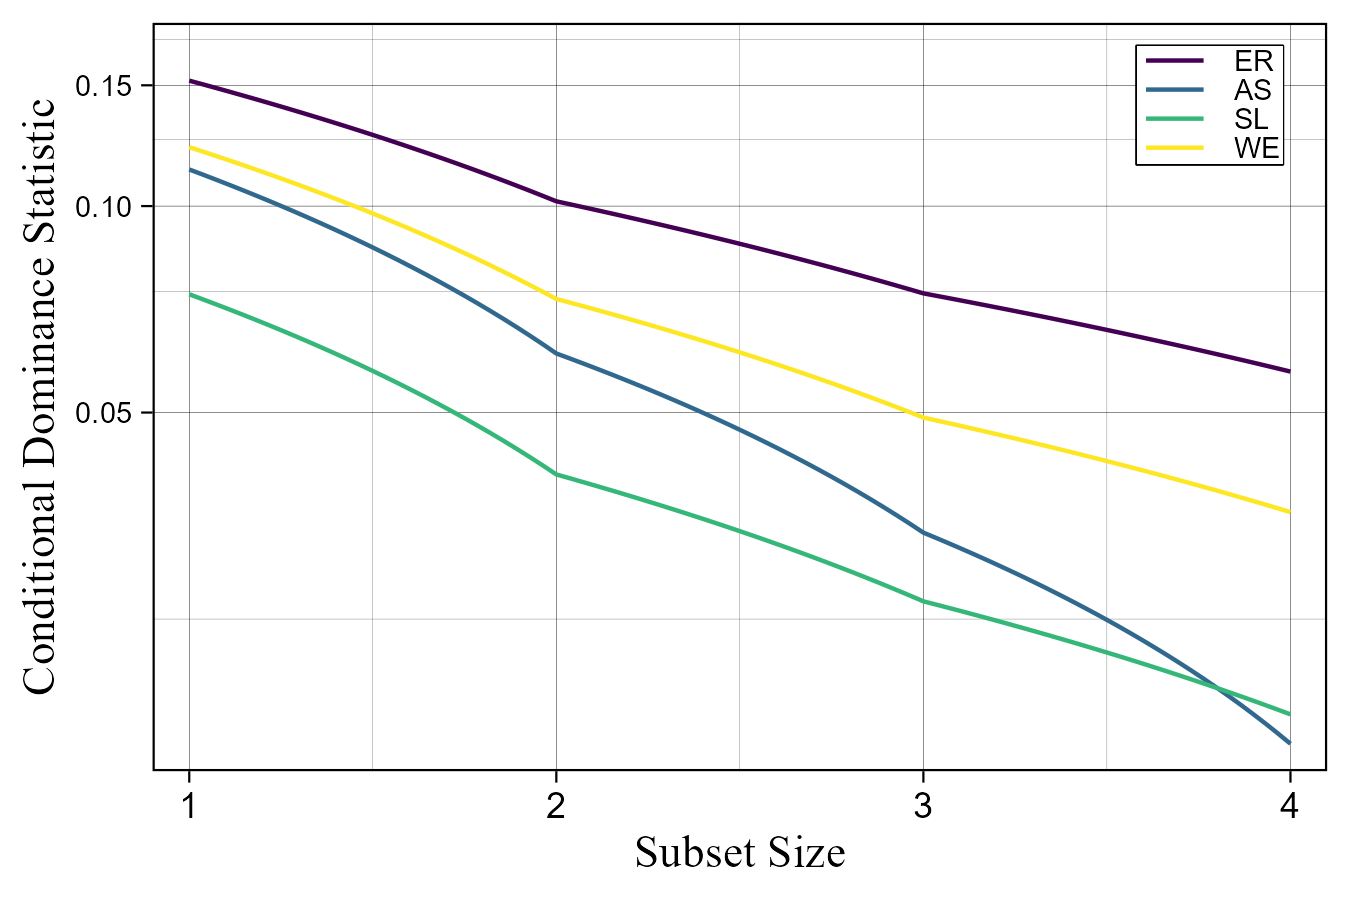
\includegraphics{condit_gph}
		\label{fg:cdl}
	\end{figure}

	I used a graphical format to depict the conditional dominance statistics' values as this format more clearly conveys the dominance designations between independent variables than does a table of values. 
	In the graphic, the orientation of each independent variable's conditional dominance statistic trendline relative to other independent variables trendlines represented the information conveyed by Equation \ref{eq:cdldom}.
	Specifically, when an independent variables conditional dominance trendline was always above another independent variable's conditional dominance trendline, the independent variable that was above conditionally dominated the one below.
	
	The trendlines in Figure \ref{fg:cdl} confirmed the complete dominance results in that equipment reliability's trendline was above the trendlines for the other three independent variables indicating that it conditionally dominated each of them.
	Similarly, work experience's trendline was above skill level's trendline consistent with the complete dominance results.
	In addition, work experience's trendline was above assistant staffing's trendline indicating that it conditionally dominated assistant staffing.
	Although work experience did not explain more information than assistant staffing in all comparable models (see $solutions \sim motivation + tact$ versus $solutions \sim tact + skill$'s in Table \ref{tab:r2sub}), when considering the average information explained given inclusion order, work experience produced bigger increments to the $R^2_{DEV}$ than did assistant staffing levels. 
	As such, work experience's dominance of assistant staffing was model dependent, but not generally dependent on independent variable inclusion order.
	
	The last two independent variables did not result in conditional dominance designation as assistant staffing failed to conditionally dominate skill level given skill level's conditional dominance statistic when included last in the model (i.e., at subset size 4) was larger than assistant staffing's statistic when included last in the model.
	These conditional dominance results further reinforce the idea that attempting to rank these independent variables is not straightforward and their contributions to prediction depend on the order of their inclusion in the model. 
	
	Given that no complete or conditional dominance designations were possible for comparing assistant staffing with skill level, I proceeded to evaluate the general dominance designations between these variables. 
	The general dominance statistics for each tailoring shop independent variable was computed using Equation \ref{eq:genst} as reported in Table \ref{tab:gen}.
	
	\begin{table}[h!]
		\centering
		\caption{\centering General Dominance Statistics}
		\begin{tabular}{l|r}
			\hline 
			$ability$ & $0.0965$ \\ 
			$motivation$ & $0.0560$ \\ 
			$tact$ & $0.0399$ \\ 
			$skill$ & $0.0700$ \\ 
			\hline 
		\end{tabular}
		\label{tab:gen}
	\end{table}

	Evaluating the general dominance designations determined by the general dominance statistics in Table \ref{tab:gen} using Equation \ref{eq:gendom} again showed that equipment reliability dominated each other variable and that work experience dominated skill level and assistant staffing. 
	A useful addition that general dominance designations added was in determining general dominance between assitant staffing and skill level.
	The general dominance designations then added to the previous dominance results in that they were the final component needed to construct an importance hierarchy among the independent variables.
	In combination, the results across all three dominance designations resulted in a clear rank ordering of the tailoring shop independent variables in predicting sport jackets: equipment reliability was most important followed by work experience, then assistant staffing, and skill level was least important.
	
	In conclusion, the DA results have built on and extended the coefficient reporting in Table \ref{tab:poisreg} by adding additional information about each of the tailoring shop independent variables' predictions.
	In particular, the dominance results offered conclusive evidence for differences between independent variables in their ability to explain variation or information in the sport jacket production variable. 
	The DA results supported the inference about the predictive usefulness of equipment reliability given its large IRR value. 
	The DA results showed that, regardless of the order in which equipment reliability might be included in the model, it always produced the biggest increment to the $R^2_{DEV}$. 
	In addition, equipment reliability was associated with nearly one-third (i.e., $\frac{.0965}{.2624} \approx \frac{1}{3}$) of the explained information in sport jackets.
	The DA results also provided useful contextualization of work experience, assistant staffing levels, and skill level.
	These three independent variables obtained similar IRR values, each within .01 of one another, which made their dominance hierarchy less easy to guess at the outset.
	The dominance designations obtained showed that the hierarchy between these variables was indeed more nuanced as work experience completely dominated only skill level and conditionally dominated assistant staffing levels. 
	Moreover, assistant staffing levels only generally dominated skill level.
	The DA results then provided useful additional information to a researcher about the differences in strength of prediction between these independent variables that would not be possible to have obtained only with their IRR values.
	
\section{Discussion}

	In this manuscript I have recommended a methodology for determining the relative importance of independent variables in count regression models.
	I recommend the DA methodology as an approach that is comprehensive in the information it provides about independent variable's prediction and, when using an appropriate fit statistic such as the $R^2_{DEV}$, can provide information analogous to the explained variance $R^2$ using the LRM.
	
	I have also walked the reader through an example data analysis applying Poisson regression to simulated data. 
	In walking the reader through this example, I use the recommended DA with $R^2_{DEV}$ fit statistic approach to evaluate the relative importance of four independent variables.
	This walk through of the DA has focused on the utilization of different levels of DA designation stringency and how these different levels offer different weights of evidence for the importance of the independent variables over one another in predicting the count dependent variable.
	
	By combining these two topics, this manuscript picks up where Blevins et al. \parencite*{blevins2015count} had left off by recommending the use of DA as a postestimation method to better understand count regression model predictions.
	Specifically, I recommend consulting Blevins et al's work when choosing to implement a count regression model as their decision flowchart can help you to choose the most appropriate count regression model given the nature of your data and follow the estimation of the count regression model with a DA to more better contextualize the predictions made by each independent variable.
	
	In this manuscript I have discussed many key considerations for researchers contemplating implementing DA in using count regression models, but I acknowledge that several relevant topics have not been included.
	Before closing, I discuss some noteworthy limitations and additional extensions of this work.
	
	\subsection{Limitations and Future Directions}
	
	In this work, I use only simulated data in the empirical examples.
	The use of simulated data was an intentional choice to avoid the need to work through many of the decision points outlined by Blevins et al. \parencite*{blevins2015count} related to the selection of an appropriate count regression model as I know the dependent variables are distibuted as Poisson or negative Binomial.
	I acknowledge that the use of the simulated data adds additional complexity to following along with the methodology in the online supplement.
	That said, all the procedures used to simulate the various count dependent variables are fully replicable, well-documented, and available as a markdown that can be used by interested readers with a working knowledge of R \parencite{R}.
	In addition, I acknowledge that only reporting the results from the Poisson regression models is a limitation.
	The Poisson regression and negative Binomial regression results were very similar and, in my view, including the negative Binomial regression results would not meaningfully add to the manucscript's narrative.
	Although the negative Binomial regression model's results are not in the manuscript, I have included the negative Binomial regression results in the supplement for interested readers.
	
	Prior work on DA has recommended that researchers use bootstrapping to estimate the reproduce-ability of dominance designations \parencite{azen2003dominance}. 
	Bootstrapping the count regression model-based dominance statistics and designations is also possible but was not examined in the present work.
	Although I have not provided an example of bootstrap reproduce-ability in this work, evaluating the bootstrap reproduce-ability of dominance designations is a useful and important practice.
	Evaluating reproduce-ability allows researchers assess a level of confidence that specific designations between independent variables will hold under resampling.
	Thus, like standard hypothesis testing, evaluating bootstrap reproduce-ability can allow a researcher to better determine whether a set of dominance designations between independent variables in a count regression model are likely to generalize beyond the sample at hand.
	
	In addition, zero inflation is commonly observed of count dependent variables.  
	Zero inflation is a condition where the distribution of the count dependent variable has more 0s than would be expected given a standard Poisson or negative Binomail distribution and requires the use of specialized models \parencite[e.g.,][]{blevins2015count, bhaskar2023regression}. 
	Cameron and Windmeijer \parencite*{cameron1996r} discuss the application of the $R^2_{DEV}$ to zero-inflated count regression models and, thus, a DA methodology based on the same general approach as discussed above could be applied to zero-inflated count regression models.
	One additional complication that arises with considering how to determine importance with zero-inflated count regression models is that these models encompass two predictive processes. 
	The first process is the standard count generating process whereby independent variables increase or decrease dependent variable counts.
	The second is an "opt out" process whereby independent variables increase or decrease the likelihood of the count being 0.
	These two processes add complexity in that they can be modeled differently. 
	Any one independent variable can predict the count generating process, the opting out process, or both.
	When using a DA with zero-inflated count regression models, I recommend the researcher consider whether they are truly interested in determining the importance of independent variables or are actually interested in determining the importance of parameter estimates \parencite{luchman2020relative}. 
	The key difference between the two perspectives is that, if one independent variable is included in both the count and opt out process, the independent variable approach would ascribe the independent variable a single set of dominance statistic designations whereas the parameter estimate perspective would break the designations into one focused on the independent variable's effect in the count process and, separately, the independent variable's effect in the opt out process.
	
	\subsection{Conclusion}
	
	DA is a useful post-estimation methodology for determining the importance of independent variables in statistical models such as count regression models.
	This manuscript has provided a recommended methodology for extending DA to count regression models and offered an extensive data analytic example focusing on the interpretation of DA statistics and designations with simulated data.
	In combination, the conceptual discussion of DA and count regression models when paired with the empirical example in this paper, will provide scientists with useful tools they can use to better understand the results of count regression models they estimate in support of research questions with count data.

\printbibliography
	
\end{document}

input{CountDominance.bbl}